\documentclass[a4paper,twoside]{book}      % Comments after  % are ignored
\begin{document}
\title{TUD Palladian Overview}

\chapter{Sample File}
In this \textbf{sample file} we discuss how easy it is to use latexToHtml.

First, some headlines:

\section{Section}
\subsection{Subsection}
\subsubsection{Subsubsection}
\subsubsection{Paragraph}
\paragraph{Paragraph}
\subparagraph{Subparagraph}

\label{sec:equation}
\section{Equations} 

Equations can be written line such as $x = 3 + 5$, or you can use the equation environment as shown in Equation~\ref{eqn:sample}.

\begin{equation}
\label{eqn:sample}
\frac{1+sin(x)}{y}
\end{equation}

\thiswontshow

\section{Footnotes}  
Footnotes\footnote{Footnotes are information about the annotated word/phrase} will be underlined and the information shows when hovering over them\footnote{You can also put URLs such as \url{http://palladian.ws} in footnotes}.

\section{Images}
Images, such as Figure \ref{fig:sample} can be added too. Figure \ref{fig:samplePng} shows a png file. 

\begin{figure}
\centering

\includegraphics[width=4in]{pngFigure.png}
\caption{Sample PNG Figure}
\label{fig:samplePng}
\end{figure}

Figure \ref{fig:samplePdf} shows an embedded pdf file.
 
\begin{figure}
\centering
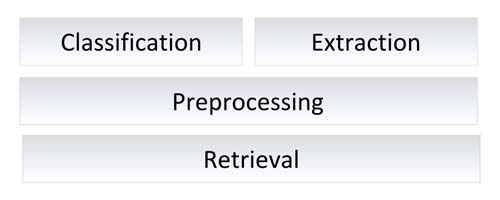
\includegraphics[width=4in]{pdfFigure.pdf}
\caption{Sample PNG Figure}
\label{fig:samplePdf}
\end{figure}

\section{Styles}
You can write \textbf{bold}, \textit{italic}, \emph{emphasize} stuff, or \verb#verbatim# as markup. Also the verbatim area as shown below is available..

\begin{verbatim}
function verbatim() {
  alert('Verbatim rocks');
}
\end{verbatim}

\section{Lists}
Lists can be used as well. Numbered (enumerate) and unordered lists (itemize) are available.

\begin{enumerate}
\item First \textbf{item}.
\item You can have equations in lists $x = 3 + 5$.
\item Last item \url{http://palladian.ws}.
\end{enumerate} 

\begin{itemize}
\item This list
\item is
\item unordered.
\end{itemize} 

\section{Tables}
Tables such as Table \ref{tab:sampleTable} are supported. Weird\footnote{Tabularx or Longtables for example} tables are not supported.

\begin{table}
\centering
\begin{tabular}{|l|c|c|c|}
	\hline
	System & Short Texts & Medium Texts & Long Texts \\ 
	\hline
	JLangDetect & \textbf{74.64\%} & 87.91\% & 99.64\% \\ 
	\hline
	Alchemy API & (97.78\%) & 69.35\% & (88.27\%) \\ 
	\hline
	Google API & 57.32\% & 80.44\% & (99.21\%) \\ 
	\hline
	Palladian & 62.36\% & \textbf{88.18\%} & \textbf{99.91\%}  \\ 
	\hline
\end{tabular}
\caption{Sample Table.}
\label{tab:sampleTable}
\end{table}

\section{Links}
Links such as URLs to external sources \url{http://palladian.ws} are supported but also anchors in the document work well (ref and label). See Section \ref{sec:equation} for example.

\section{Citations}
Citations \cite{palladian2012} are partially supported.


\end{document}
